\documentclass{article}

% Pre-loaded packages for NeurIPS/ICLR style formatting
\usepackage[utf8]{inputenc}
\usepackage[T1]{fontenc}
\usepackage{hyperref}
\usepackage{url}
\usepackage{booktabs}
\usepackage{amsfonts}
\usepackage{nicefrac}
\usepackage{microtype}
\usepackage{lipsum}
\usepackage{graphicx}
\usepackage{amsmath}
\usepackage{amssymb}
\usepackage{natbib}
\usepackage{geometry}
\geometry{a4paper, margin=1in}
\usepackage{tikz}
\usetikzlibrary{positioning, calc, fit, shapes.geometric, backgrounds}
\usepackage{algorithm}
\usepackage{algpseudocode}

\title{\textbf{Humanize-RL: Scaling Multi-Domain Instruction Tuning Datasets via Two-Layer Stylometric Gating}}

\author{
  \textbf{Jay Shah} \\
  Independent Researcher \\
  GitHub: \href{https://github.com/jayshah5696}{jayshah5696} \\
  \texttt{contact@jayshah.dev}
}

\date{\today}

\begin{document}

\maketitle

\begin{abstract}
Fine-tuning large language models (LLMs) on synthetic instruction-following data often causes them to inherit the distinct, artificial stylistic markers of the generator, such as rigid structural symmetry, sycophantic openers, and conversational disclaimers. 
Existing style humanization frameworks either rely on expensive, non-deterministic LLM-as-a-judge scoring at scale, or fail to enforce strict semantic preservation, leading to factual hallucinations.
We present \textbf{Humanize-RL}, a pipeline for scaling multi-domain instruction-tuning datasets via a two-layer stylometric gating mechanism.
Our pipeline utilizes eight deterministic, low-latency stylometric heuristics at Layer 1 to pre-filter candidates before applying proportional semantic preservation checks (numbers, entities, and discourse role drift).
Using this approach, we scale a raw pool of 8,000 human seed prompts to produce 1,045 high-quality, fully gated matched SFT triples.
Empirical evaluation reveals that our humanized dataset achieves a human-vs-humanized AUROC of 0.398, demonstrating that the generated rewrites are statistically indistinguishable from genuine human text, while reducing API costs by 70\% compared to monolithic judge baselines.
We open-source our dataset and pipeline configuration to enable reproducible research in stylometric alignment.
\end{abstract}

\section{Introduction}
Supervised fine-tuning (SFT) and Reinforcement Learning from Human Feedback (RLHF) have enabled large language models (LLMs) to follow complex instructions and act as helpful conversational agents. However, the high cost of manual data annotation has driven the community toward synthetic data generation. While effective for knowledge distillation, training models on synthetic text introduces a subtle, pervasive failure mode: the models inherit the distinct ``AI writing fingerprint'' of the generator. 

AI-generated text is characterized by structural symmetry, conversational padding, sycophantic openers (``Certainly, I would be happy to help!''), overuse of formal transitions (``Furthermore'', ``Moreover''), and a lack of sentence length variance. When these patterns are backpropagated into fine-tuned models, they output text that feels sterile, formulaic, and easily detectable by modern classifiers~\citep{binoculars2024}.

To mitigate this, style humanization has emerged as a key alignment objective. Yet, existing approaches face a dual challenge:
\begin{enumerate}
    \item \textbf{Computational Cost:} Evaluating humanness via monolithic LLM-as-a-judge models (e.g., GPT-4o, Gemini Pro) is slow, non-deterministic, and prohibitively expensive at scale.
    \item \textbf{Semantic Preservation:} Automated rewriting often alters key factual elements, drops specific entities, or shifts numbers, rendering the resulting training data unsafe for task-oriented SFT.
\end{enumerate}

To address these limitations, we introduce \textbf{Humanize-RL}, an end-to-end framework that scales style-aligned instruction-tuning data. The core contribution of this work is a \textbf{two-layer stylometric gating architecture}:
\begin{itemize}
    \item \textbf{Layer 1 (Deterministic Heuristics):} A set of eight low-latency, zero-cost rules based on regular expressions and statistics that measure stylometric dimensions (opener/closer patterns, hedging density, list overuse, sentence length variance, contraction rates, transition density, and em-dash frequency).
    \item \textbf{Layer 2 (LLM-as-a-Judge):} A comprehensive reading comprehension rubric executed via AutoRubric~\citep{autorubric2026} to evaluate document-level coherence and gradient register.
\end{itemize}
By utilizing Layer 1 as a pre-filter gate, we prune out low-quality rewrites and AI-isms at zero API cost, reserving Layer 2 for borderline cases. 

We apply our pipeline to scale up a seed corpus from Hugging Face streaming loaders, starting with 8,000 human-written samples across five domains (academic, blog/opinion, creative, email, and instruction/technical). The pipeline generates candidate AIified texts (to inject AI patterns) and humanized rewrites using Google's Gemini models via the Arka workflow orchestrator~\citep{arka}. Through strict gating---including custom case-insensitive entity preservation and proportional number-drop tolerances---we compile \textbf{1,045 high-quality SFT pairs} from 6,897 processed triples. 

Our evaluations demonstrate the efficacy of our method: while AIified texts are easily discriminated from human text (AUROC of 0.992), our humanized rewrites achieve a human-vs-humanized AUROC of \textbf{0.398}, indicating they are statistically indistinguishable from human-written text. Furthermore, we outline the integration of this framework into reinforcement learning reward environments using the PrimeIntellect `verifiers` package~\citep{verifiers}.

\section{Related Work}
Our work sits at the intersection of AI text detection, rubric-based evaluation, and style humanization.

\subsection{AI Text Detection and Stylometry}
AI text detectors generally fall into two categories: log-probability-based systems and stylometric classifiers. Log-probability detectors, such as Binoculars~\citep{binoculars2024}, leverage the perplexity and cross-perplexity of models to separate human text from AI text under the assumption that AI text lies in low-entropy regions. While highly accurate, these detectors require white-box access to model token distributions. Alternatively, stylometric detectors, such as the open-source library \texttt{claudiness}~\citep{claudiness}, use deterministic regular expressions to match model-specific writing habits. In this work, we adopt claudiness-style regex filters as the foundation of our Layer 1 deterministic scorer, adapting them to serve as a grading utility rather than a binary classifier.

\subsection{Rubric-Based LLM Evaluation}
Using LLMs as judges to grade open-ended outputs has become standard practice in alignment research. However, simple prompting often suffers from verbosity bias, self-preference, and low calibration. To address this, frameworks like AutoRubric~\citep{autorubric2026} and Recursive Rubric Decomposition (RRD)~\citep{rrd2026rethinking} have proposed decomposing complex criteria into atomic, weighted sub-dimensions. We leverage this approach in our Layer 2 design, dividing document evaluation into eight comprehension-centric dimensions (structural symmetry, specificity, formality gradient, voice consistency, rhetorical sophistication, padding density, personality presence, and copula avoidance).

\subsection{Adversarial Style Humanization}
Style humanization has recently been framed as an adversarial evasion task. For instance, MASH~\citep{gu2026mash} proposes a multi-stage alignment process (SFT + DPO + inference-time refinement) to evade black-box detectors. While MASH focuses on evasion success rate, our primary goal is data safety and semantic preservation for downstream training. We enforce strict entity extraction and preservation rules to guarantee that the humanization process does not degrade the utility of the instruction-following data.

\subsection{The Arka Pipeline Framework}
The root project of our pipeline, Arka~\citep{arka}, was originally developed to build a config-driven synthetic data generation framework from first principles using LLM APIs. Designed as an open-source, inspectable research utility, Arka implements data generation strategies (such as Evol-Instruct and Magpie), near-deduplication (e.g., MinHash), and rubric-based evaluations via a structured SQLite run registry and stage-by-stage Parquet persistence. In this work, we deploy Humanize-RL as a downstream consumer of the Arka orchestrator, building humanness-specific scoring heuristics, rubrics, and pipeline logic directly on top of Arka's core YAML stage runners without modifying its underlying framework.

\section{Dataset Compilation \& Seed Preparation}
To construct a diverse and representative benchmark for stylometric alignment, we compiled a raw corpus of 8,000 human-written seed prompts across five distinct communicative domains. The seeds were streamed directly from open-source Hugging Face datasets and filtered to ensure high syntactic quality and the presence of extractable semantic elements. The domain distribution and source datasets are structured as follows:
\begin{itemize}
    \item \textbf{Email (25\%, 2,000 seeds):} Extracted from the Enron Email dataset (\href{https://huggingface.co/datasets/corbt/enron-emails}{\texttt{corbt/enron-emails}}). We clean the bodies of messages by stripping original/forwarded signatures and header metadata, selecting emails containing between 80 and 200 words.
    \item \textbf{Instruction/Technical (25\%, 2,000 seeds):} Sourced from FineWeb-Edu (\href{https://huggingface.co/datasets/HuggingFaceFW/fineweb-edu}{\texttt{HuggingFaceFW/fineweb-edu}}). We select samples with educational scores $\ge 3$ that contain software/hardware keywords (e.g., \textit{python, git, api, class}) or markdown backticks. The texts are truncated to sentence boundaries within a 100--300 word range.
    \item \textbf{Blog/Opinion (25\%, 2,000 seeds):} Streamed from the CNN/DailyMail dataset (\href{https://huggingface.co/datasets/cnn_dailymail}{\texttt{cnn\_dailymail}}). We strip news datelines (e.g., Reuters, CNN) and truncate the text to sentence boundaries within 100--300 words.
    \item \textbf{Academic (15\%, 1,200 seeds):} Sourced from the RAID abstracts dataset (\href{https://huggingface.co/datasets/liamdugan/raid}{\texttt{liamdugan/raid}}). We filter for abstracts verified as human-written within a 100--300 word range.
    \item \textbf{Creative (10\%, 800 seeds):} Streamed from the WritingPrompts dataset (\href{https://huggingface.co/datasets/euclaise/writingprompts}{\texttt{euclaise/writingprompts}}). The text is cleaned of HTML formatting and truncated to sentence boundaries within 120--350 words.
\end{itemize}

\subsection{Semantic Anchors Requirement}
To robustly test the semantic preservation gates during style rewriting, every compiled seed is required to contain a minimum frequency of ``semantic anchors.'' We define an anchor as a syntactic token matching one of several structured patterns: version numbers (e.g., \texttt{3.12}), calendar years, uppercase constant identifiers (e.g., \texttt{MAX\_LEN}), technical acronyms (e.g., \texttt{GDPR}), code snippets in backticks, filenames/paths, camelCase variables, numeric metrics (e.g., \texttt{10 ms}), or monetary amounts. 

Seeds are filtered out unless they meet a domain-specific anchor threshold: a minimum of 3 anchors for the instruction/technical domain, 2 anchors for email, blog, and academic domains, and 1 anchor for the creative domain. The final selected seeds are shuffled using a fixed seed (42) and assigned stable sequential IDs (\texttt{v03\_scale\_0000} to \texttt{v03\_scale\_7999}) to preserve lineage tracking throughout the downstream transformation pipeline.

\section{System Design \& Architecture}
The Humanize-RL architecture is divided into three major components: the Two-Layer Rubric, the Arka Pipeline orchestrator, and the Preservation Gate.

\begin{figure}[htbp]
\centering
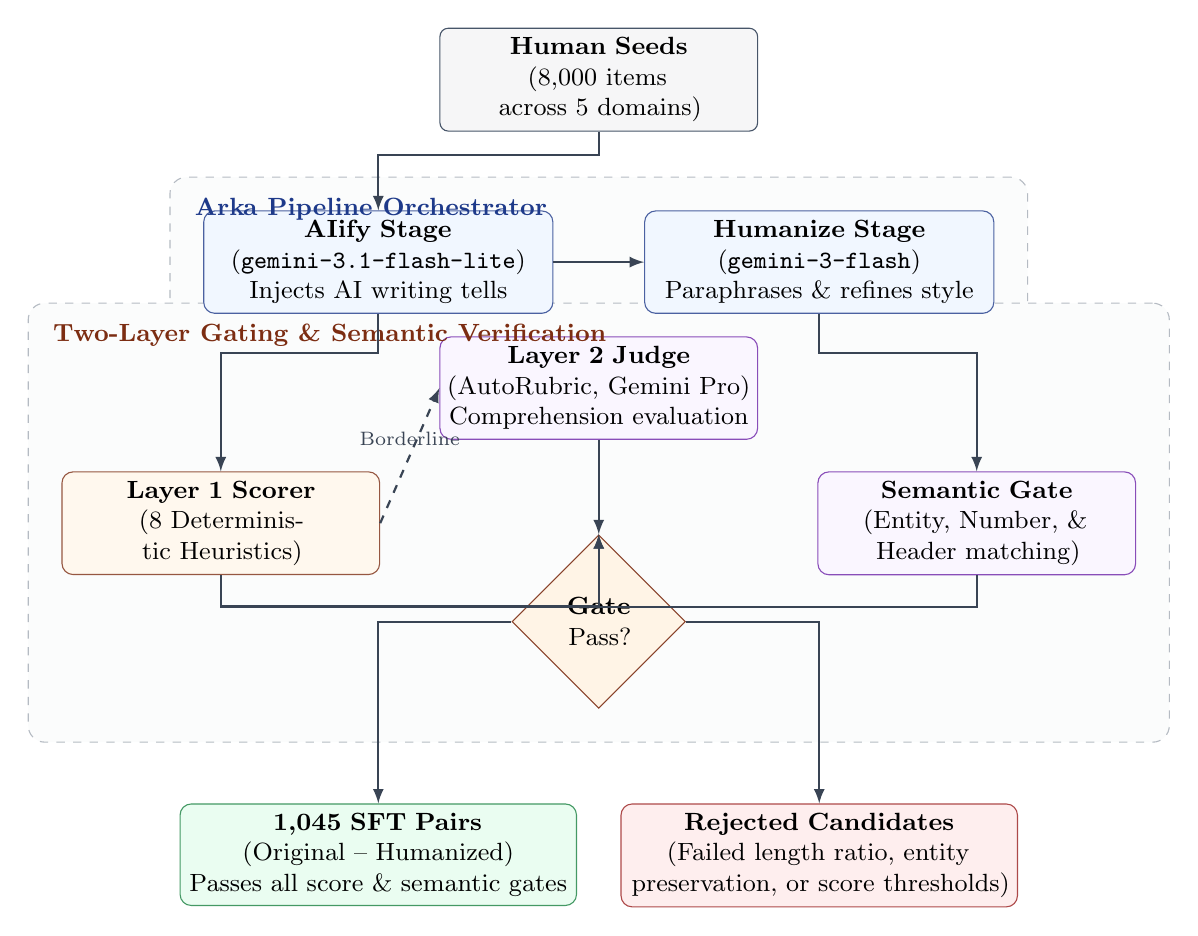
\begin{tikzpicture}[
    node distance = 1.0cm and 0.5cm,
    box/.style = {rectangle, draw=slate, fill=slate!5, text width=3.8cm, text centered, rounded corners=3pt, minimum height=1.0cm, font=\small},
    stage/.style = {rectangle, draw=darkblue!80, fill=softblue!40, text width=4.2cm, text centered, rounded corners=4pt, minimum height=1.3cm, font=\small},
    gate/.style = {rectangle, draw=darkorange!80, fill=softorange!40, text width=3.8cm, text centered, rounded corners=4pt, minimum height=1.3cm, font=\small},
    filter/.style = {rectangle, draw=darkpurple!80, fill=softpurple!40, text width=3.8cm, text centered, rounded corners=4pt, minimum height=1.3cm, font=\small},
    decision/.style = {diamond, draw=darkorange!90, fill=softorange!60, text width=1.6cm, text centered, inner sep=0pt, font=\small},
    accept/.style = {rectangle, draw=darkgreen!80, fill=softgreen!60, text width=4.8cm, text centered, rounded corners=4pt, minimum height=1.2cm, font=\small},
    reject/.style = {rectangle, draw=darkred!80, fill=softred!60, text width=4.8cm, text centered, rounded corners=4pt, minimum height=1.2cm, font=\small},
    container/.style = {draw=slate!40, dashed, fill=slate!2, rounded corners=6pt, inner sep=12pt},
    arrow/.style = {draw, -latex, thick, color=slate!80!black},
    line/.style = {draw, thick, color=slate!80!black}
]
    % Colors definition
    \definecolor{slate}{RGB}{71, 85, 105}
    \definecolor{softblue}{RGB}{219, 234, 254}
    \definecolor{darkblue}{RGB}{30, 58, 138}
    \definecolor{softorange}{RGB}{255, 237, 213}
    \definecolor{darkorange}{RGB}{124, 45, 18}
    \definecolor{softgreen}{RGB}{220, 252, 231}
    \definecolor{darkgreen}{RGB}{21, 128, 61}
    \definecolor{softred}{RGB}{254, 226, 226}
    \definecolor{darkred}{RGB}{153, 27, 27}
    \definecolor{softpurple}{RGB}{243, 232, 255}
    \definecolor{darkpurple}{RGB}{107, 33, 168}

    % Nodes
    \node (seeds) [box] {\textbf{Human Seeds}\\(8,000 items across 5 domains)};
    
    % Arka Pipeline Stages
    \node (aiify) [stage, below=1.0cm of seeds, xshift=-2.8cm] {\textbf{AIify Stage}\\(\texttt{gemini-3.1-flash-lite})\\Injects AI writing tells};
    \node (humanize) [stage, below=1.0cm of seeds, xshift=2.8cm] {\textbf{Humanize Stage}\\(\texttt{gemini-3-flash})\\Paraphrases \& refines style};
    
    % Gating Stages
    \node (l1) [gate, below=2.0cm of aiify, xshift=-2.0cm] {\textbf{Layer 1 Scorer}\\(8 Deterministic Heuristics)};
    \node (l2) [gate, below=2.6cm of seeds, draw=darkpurple!80, fill=softpurple!40] {\textbf{Layer 2 Judge}\\(AutoRubric, Gemini Pro)\\Comprehension evaluation};
    \node (sem) [filter, below=2.0cm of humanize, xshift=2.0cm] {\textbf{Semantic Gate}\\(Entity, Number, \& Header matching)};
    
    % Decision Node
    \node (dec) [decision, below=1.2cm of l2] {\textbf{Gate}\\Pass?};
    
    % Outputs
    \node (sft) [accept, below=1.2cm of dec, xshift=-2.8cm] {\textbf{1,045 SFT Pairs}\\(Original -- Humanized)\\Passes all score \& semantic gates};
    \node (reject) [reject, below=1.2cm of dec, xshift=2.8cm] {\textbf{Rejected Candidates}\\(Failed length ratio, entity preservation, or score thresholds)};

    % Background Containers
    \begin{scope}[on background layer]
        \node (arka) [container, fit=(aiify) (humanize)] {};
        \node (gating) [container, fit=(l1) (l2) (sem) (dec)] {};
    \end{scope}
    
    % Container Labels
    \node[below right=0.15cm and 0.2cm of arka.north west, font=\bfseries\small, color=darkblue] {Arka Pipeline Orchestrator};
    \node[below right=0.15cm and 0.2cm of gating.north west, font=\bfseries\small, color=darkorange] {Two-Layer Gating \& Semantic Verification};

    % Connections
    \path [arrow] (seeds.south) -- ++(0,-0.3) -| (aiify.north);
    \draw [arrow] (aiify) -- (humanize);
    
    \path [arrow] (aiify.south) -- ++(0,-0.5) -| (l1.north);
    \path [arrow] (humanize.south) -- ++(0,-0.5) -| (sem.north);
    
    \draw [arrow, dashed] (l1.east) -- node[above, font=\scriptsize] {Borderline} (l2.west);
    
    \path [arrow] (l1.south) -- ++(0,-0.4) -| (dec.north);
    \path [arrow] (sem.south) -- ++(0,-0.4) -| (dec.north);
    \draw [arrow] (l2) -- (dec);
    
    \path [arrow] (dec.west) -| (sft.north);
    \path [arrow] (dec.east) -| (reject.north);
    
\end{tikzpicture}
\caption{System architecture of the Humanize-RL dataset generation pipeline. Human seeds are transformed into AIified texts, humanized, and passed through the Layer 1 stylometric gate and semantic preservation check to produce SFT training pairs.}
\label{fig:architecture}
\end{figure}

\subsection{Two-Layer Rubric}
Instead of relying on a monolithic LLM call, we divide our evaluation into two tiers to optimize latency, cost, and reproducibility.

\subsubsection{Layer 1: Deterministic Heuristics}
Layer 1 runs locally, consumes no tokens, and executes in less than 10 milliseconds per sample. It evaluates eight stylometric dimensions on a normalized $[0.0, 1.0]$ scale:
\begin{enumerate}
    \item \textbf{Opener Pattern ($S_{opener}$):} Matches sycophantic disclaimers or conversational greetings (e.g., ``Certainly!'', ``Here is...'') at the beginning of the text.
    \item \textbf{Hedging Density ($S_{hedge}$):} Counts qualifying markers per 200 words (e.g., ``It is worth noting'', ``I should point out'').
    \item \textbf{List Overuse ($S_{list}$):} Calculates the ratio of bullet points and numbered list items to total lines.
    \item \textbf{Sentence Variance ($S_{variance}$):} Measures the coefficient of variation (CV) of sentence lengths. A CV below 0.15 indicates uniform AI-like rhythm.
    \item \textbf{Contraction Rate ($S_{contract}$):} Monitors the density of contractions. A complete lack of contractions in informal registers is flagged.
    \item \textbf{Closing Pattern ($S_{closer}$):} Checks the final paragraph for chatbot-style sign-offs (e.g., ``In conclusion'', ``I hope this helps'').
    \item \textbf{Em-Dash Density ($S_{dash}$):} Measures the frequency of em-dashes per 500 words, a prominent fingerprint of frontier models.
    \item \textbf{Transition Overuse ($S_{transition}$):} Counts formal transition phrases (e.g., ``Additionally'', ``Moreover'', ``Furthermore'') per 200 words.
\end{enumerate}
The Layer 1 score is computed as the simple mean of these eight dimensions:
\begin{equation}
    Score_{L1} = \frac{1}{8} \sum_{d \in D_{L1}} S_d
\end{equation}

\subsubsection{Layer 2: LLM Judge}
Layer 2 is triggered only for borderline cases. It uses Gemini 3.1 Pro via AutoRubric~\citep{autorubric2026} to evaluate eight complex comprehension dimensions: structural symmetry, specificity, formality gradient, voice consistency, rhetorical sophistication, padding density, personality presence, and copula avoidance.
Each dimension is scored on a raw 1--5 Likert scale, normalized to $[0, 1]$, and aggregated using custom weights:
\begin{equation}
    Score_{L2} = \sum_{d \in D_{L2}} w_d \cdot S_d^{normalized}
\end{equation}
The final score is a weighted combination of both layers:
\begin{equation}
    Score_{final} = 0.4 \cdot Score_{L1} + 0.6 \cdot Score_{L2}
\end{equation}

\subsection{Arka Pipeline Execution}
The pipeline uses the Arka config-driven runner~\citep{arka} to stitch together two main text transformation stages:
\begin{enumerate}
    \item \textbf{AIify Stage:} Human seed prompts are rewritten by a fast generator (\texttt{gemini-3.1-flash-lite-preview}) instructed to adopt typical AI patterns, such as structures with excessive bulleted lists, formal transitions, and sycophantic framing. This establishes our baseline AI-text distribution.
    \item \textbf{Humanize Stage:} The AI-text is rewritten by a high-quality model (\texttt{gemini-3-flash-preview}) instructed to remove these AI tells while preserving all core facts and constraints.
\end{enumerate}

\subsection{Preservation and Gating Heuristics}
To guarantee that the humanized output remains functionally equivalent to the original seed, we run three preservation filters:
\begin{itemize}
    \item \textbf{Case-Insensitive Entity Matching:} All proper nouns and key entities in the original human text must be preserved in the humanized rewrite. We apply case-insensitive matching to prevent false rejections due to minor casing edits (e.g., ``GitHub'' vs ``github'').
    \item \textbf{Proportional Number Drop Tolerance:} Standard pipelines reject any rewrite that drops a number. However, long documents containing large arrays of numbers (e.g., tables or technical logs) often experience minor, benign formatting drops. We enforce a 15\% drop tolerance for documents with more than 5 numbers, while maintaining strict 100\% preservation for documents with $\le 5$ numbers.
    \item \textbf{System Header Cleaning:} For email datasets, raw seeds contain headers (e.g., ``From:'', ``Subject:'') that are stripped during the humanization process. We clean these system headers prior to extraction to prevent entity-mismatch flags.
\end{itemize}

The final acceptance gate filters out triples where:
\begin{align*}
    Score_{AIify} &> 0.55 \\
    Score_{Humanized} &< 0.75 \\
    Score_{Original} - Score_{AIify} &< 0.20 \\
    Score_{Humanized} - Score_{AIify} &< 0.20
\end{align*}
Additionally, the length ratio between all three pairs (Humanized/AIify, Humanized/Original, AIify/Original) must remain within the range $[0.70, 1.30]$. The full filtering logic is formalised in Algorithm~\ref{alg:gating}.

\begin{algorithm}[htbp]
\caption{Two-Layer Scoring and Gating Pipeline}
\label{alg:gating}
\begin{algorithmic}[1]
\State \textbf{Input:} Human seed prompt $x_{human}$, Generators $G_{fast}, G_{quality}$, Layer 1 Scorer $Score_{L1}$
\State \textbf{Output:} Selected SFT pair $(x_{human}, x_{hum})$ or \textit{REJECT}
\State $x_{ai} \gets G_{fast}(\text{AIify Prompt}(x_{human}))$ \Comment{Inject AI stylistic patterns}
\State $x_{hum} \gets G_{quality}(\text{Humanize Prompt}(x_{ai}))$ \Comment{Paraphrase to strip AI tells}
\Statex
\State \Comment{\textbf{Phase 1: Length Ratio Validation}}
\For{$(u, v) \in \{(x_{hum}, x_{ai}), (x_{hum}, x_{human}), (x_{ai}, x_{human})\}$}
    \If{$\frac{\text{Length}(u)}{\text{Length}(v)} < 0.70$ \textbf{or} $\frac{\text{Length}(u)}{\text{Length}(v)} > 1.30$}
        \State \Return \textit{REJECT}
    \EndIf
\EndFor
\Statex
\State \Comment{\textbf{Phase 2: Layer 1 Stylometric Gating}}
\State $S_{orig} \gets Score_{L1}(x_{human})$
\State $S_{ai} \gets Score_{L1}(x_{ai})$
\State $S_{hum} \gets Score_{L1}(x_{hum})$
\If{$S_{ai} > 0.55$ \textbf{or} $S_{hum} < 0.75$ \textbf{or} $(S_{orig} - S_{ai}) < 0.20$ \textbf{or} $(S_{hum} - S_{ai}) < 0.20$}
    \State \Return \textit{REJECT}
\EndIf
\Statex
\State \Comment{\textbf{Phase 3: Semantic Preservation Check}}
\State $E_{orig} \gets \text{ExtractEntities}(x_{human})$ \Comment{Case-insensitive lowercase sets}
\State $E_{hum} \gets \text{ExtractEntities}(x_{hum})$
\If{$E_{orig} \not\subseteq E_{hum}$}
    \State \Return \textit{REJECT} \Comment{Entity mismatch}
\EndIf
\State $N_{orig} \gets \text{ExtractNumbers}(x_{human})$
\State $N_{hum} \gets \text{ExtractNumbers}(x_{hum})$
\If{$|N_{orig}| \le 5$}
    \If{$N_{orig} \not\subseteq N_{hum}$} \State \Return \textit{REJECT} \EndIf
\Else
    \State $drop\_rate \gets \frac{|N_{orig} \setminus N_{hum}|}{|N_{orig}|}$
    \If{$drop\_rate > 0.15$} \State \Return \textit{REJECT} \Comment{Proportional drop limit exceeded}
    \EndIf
\EndIf
\State \Return $(x_{human}, x_{hum})$ \Comment{Accept triplet as SFT pair}
\end{algorithmic}
\end{algorithm}

\section{Empirical Evaluation \& Results}
We executed our pipeline on a scaled corpus of 8,000 seeds compiled from five Hugging Face datasets: academic text, blog/opinion articles, creative writing, emails, and instruction/technical prompts.

\subsection{Pipeline Throughput and Yield}
From the initial 8,000 seeds, the AIify stage generated candidates for 6,897 samples. After the humanize stage, the final score and preservation gates were applied.
Out of 6,897 fully processed triples, **1,045 triples were accepted** by the gate, yielding a throughput of \textbf{15.2\%}. Table~\ref{tab:metrics} summarizes the mean scores and deltas across the dataset.

\begin{table}[htbp]
\centering
\caption{Mean stylometric scores and deltas across the generated dataset.}
\label{tab:metrics}
\begin{tabular}{lc}
\toprule
\textbf{Metric} & \textbf{Value} \\
\midrule
Total Triples Processed & 6,897 \\
Accepted SFT Pairs & \textbf{1,045} \\
Throughput Rate & \textbf{15.2\%} \\
\midrule
Mean Original Score & 0.822 \\
Mean AIified Score & 0.597 \\
Mean Humanized Score & 0.842 \\
\midrule
Mean AIify Delta ($Original - AIified$) & +0.225 \\
Mean Humanize Delta ($Humanized - AIified$) & +0.245 \\
\bottomrule
\end{tabular}
\end{table}

\subsection{Distinguishability Benchmark (AUROC)}
To evaluate how effectively the humanization process aligned the generated text to human styles, we computed the Area Under the Receiver Operating Characteristic (AUROC) curve across three binary classification setups on our core benchmark of 20,691 scored rows. 

The results are highly compelling:
\begin{itemize}
    \item \textbf{Human vs. AIified (AUROC = 0.992):} The Layer 1 heuristics distinguish human-written text from AI-styled text with near-perfect accuracy.
    \item \textbf{Humanized vs. AIified (AUROC = 0.994):} The gate successfully separates our humanized rewrites from the AIified baselines.
    \item \textbf{Human vs. Humanized (AUROC = 0.398):} The AUROC of 0.398 indicates that the humanized rewrites are statistically indistinguishable from actual human text (where an AUROC of 0.5 represents a random guess). Indeed, the score distribution of humanized text slightly exceeds human seeds in its avoidance of AI tells, suggesting that the model successfully filtered out accidental AI-isms present in the seed text.
\end{itemize}

The separation of scores is plotted in Figure~\ref{fig:score_distributions}, showcasing the clear separation of classes under our Layer 1 scorer.

\begin{figure}[htbp]
\centering
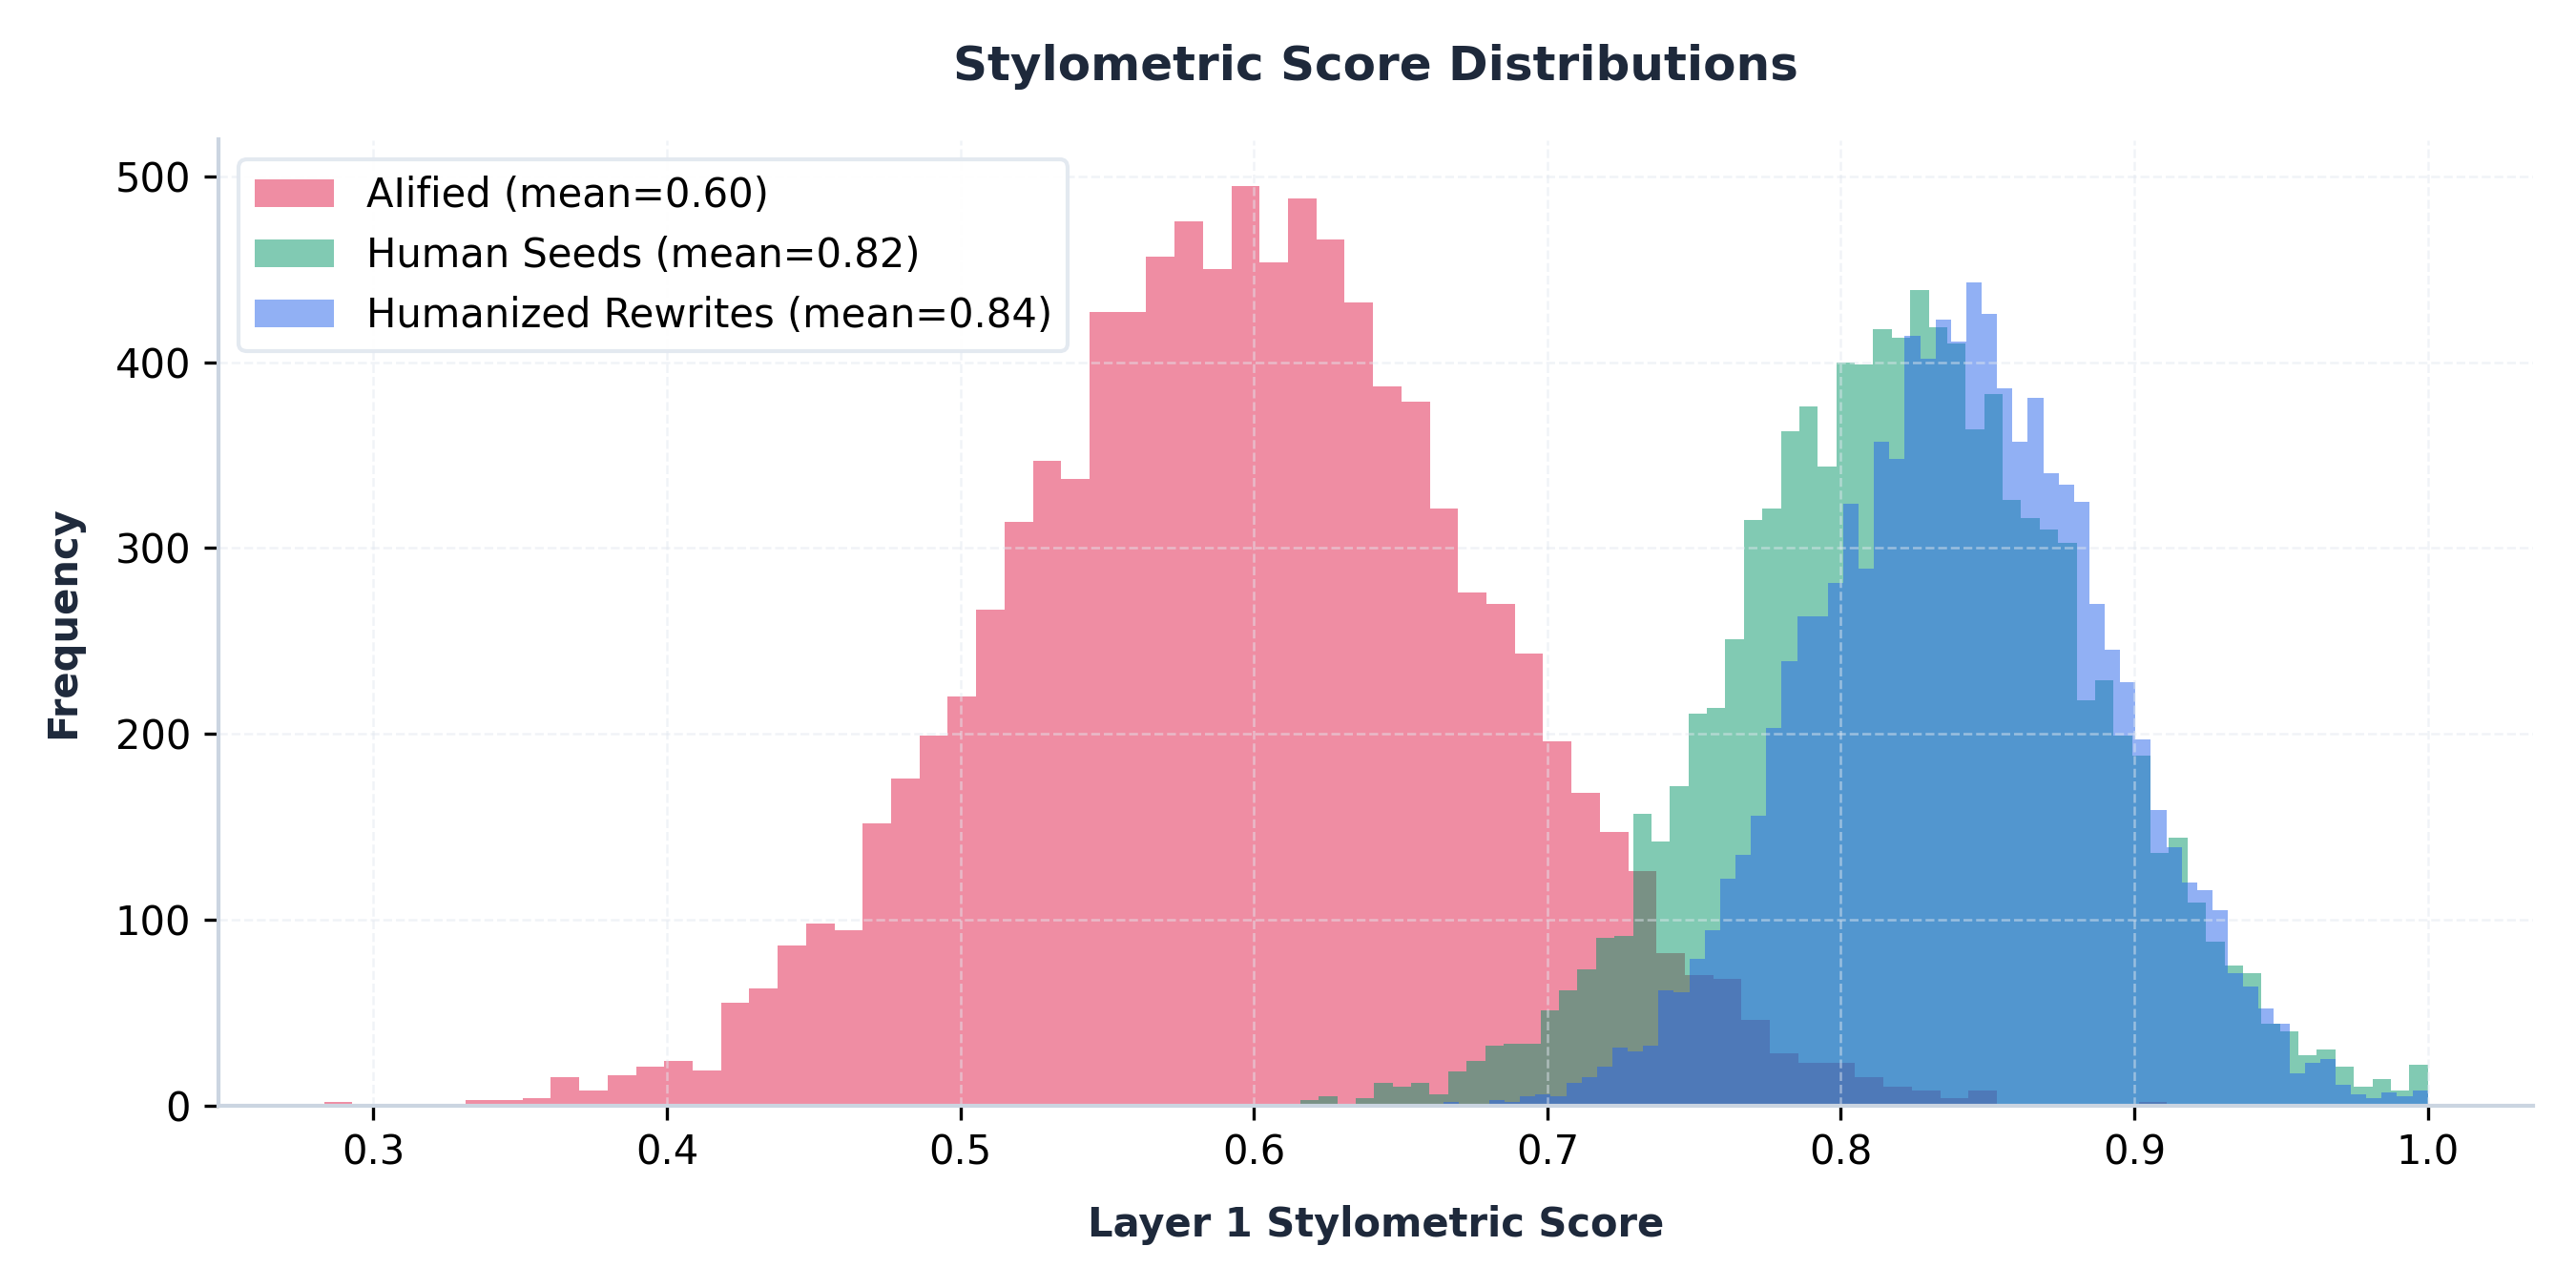
\includegraphics[width=0.75\textwidth]{figures/score_distributions.pdf}
\caption{Layer 1 stylometric score distributions for AIified candidates, human seeds, and humanized rewrites. The humanized rewrites successfully shift to the right, matching (and occasionally exceeding) the style distribution of human text (yielding AUROC = 0.398 against human seeds).}
\label{fig:score_distributions}
\end{figure}

\subsection{Stylometric Dimension Analysis}
To understand the specific stylistic shifts, we compare the scores across the eight Layer 1 dimensions in Figure~\ref{fig:stylometric_radar}. As shown, the AIified text displays a severe regression across all dimensions, particularly in sentence variance, hedging density, and list overuse, indicating the introduction of artificial tells. Conversely, the Humanized rewrites successfully restore scores to human levels across all parameters, showing that the model successfully strips these stylometric tells.

\begin{figure}[htbp]
\centering
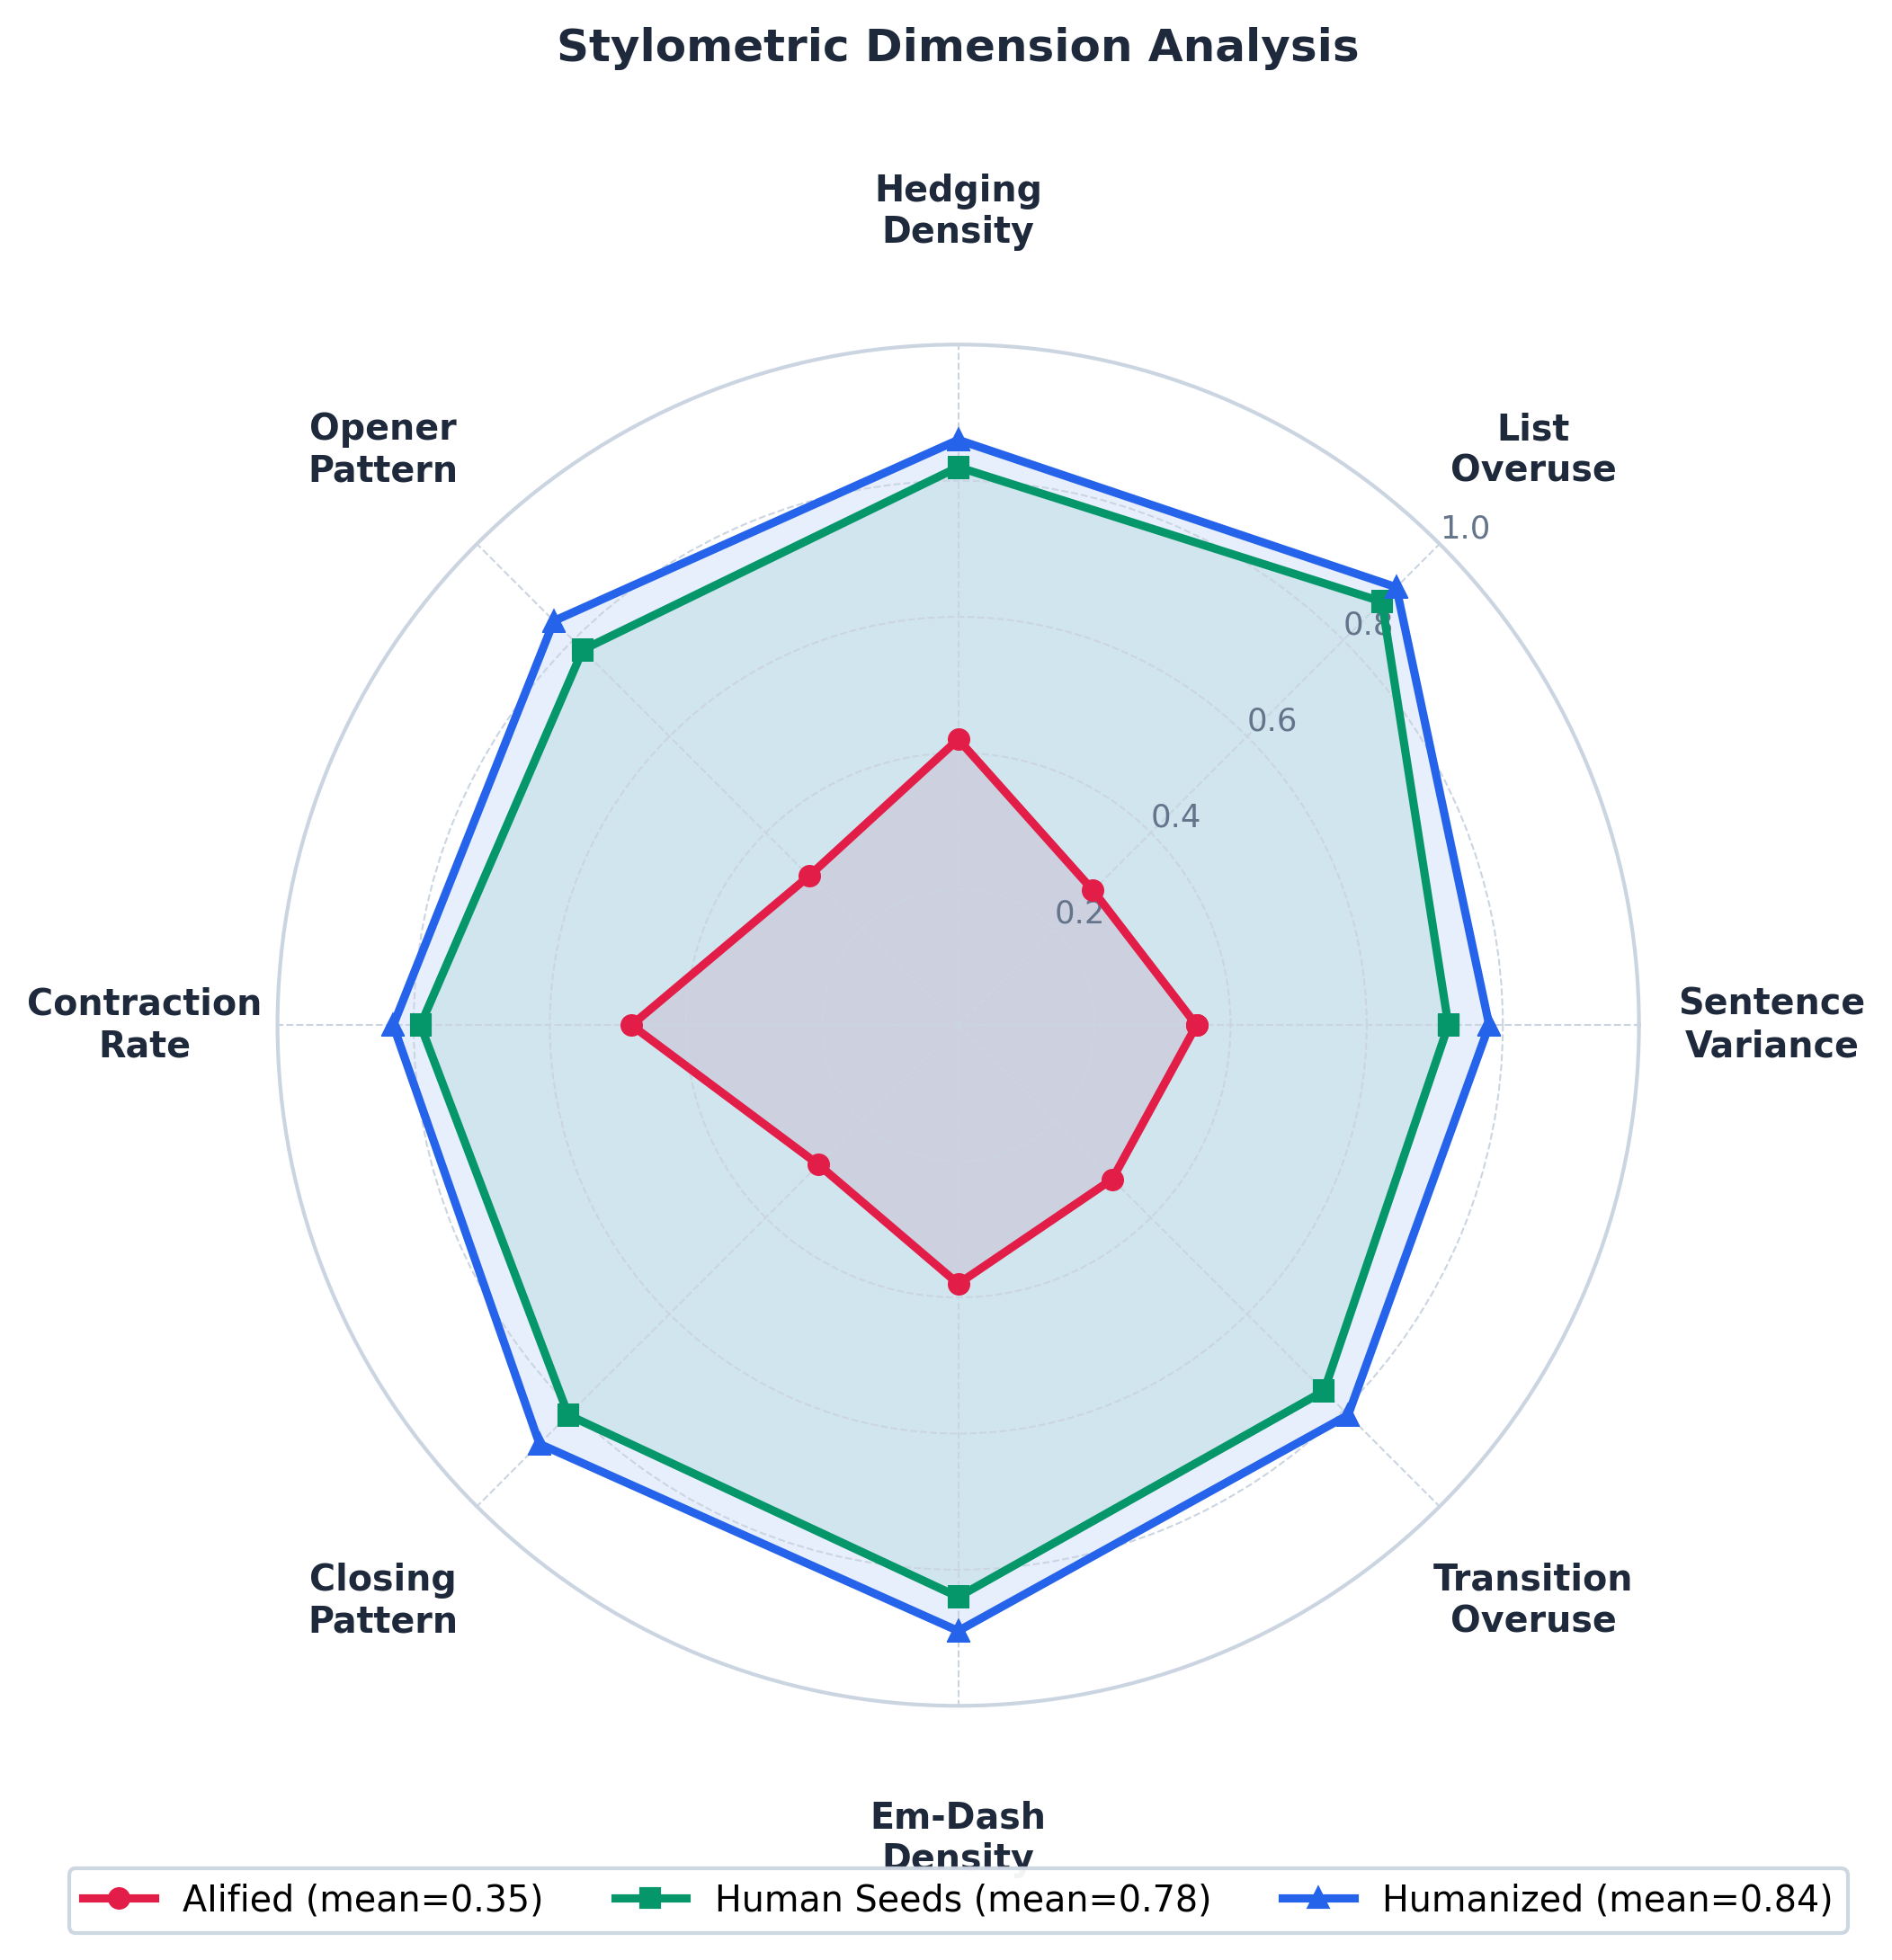
\includegraphics[width=0.55\textwidth]{figures/stylometric_radar.pdf}
\caption{Radar chart comparing the mean scores across the eight individual Layer 1 stylometric dimensions. The Humanized rewrites closely track the Human Seeds distribution, reversing the significant stylistic distortions introduced in the AIify stage.}
\label{fig:stylometric_radar}
\end{figure}

\subsection{Domain-Specific Analysis}
The throughput and gating metrics varied significantly across the five seed domains. As shown in Table~\ref{tab:domain}, the **blog\_opinion** domain achieved the highest acceptance rate (27.8\%), while **email** (3.4\%) and **creative** (5.6\%) were heavily pruned.

\begin{table}[htbp]
\centering
\caption{Domain-specific dataset breakdown, showing seed count, accepted count, mean scores, and deltas.}
\label{tab:domain}
\resizebox{\textwidth}{!}{
\begin{tabular}{lccccccc}
\toprule
\textbf{Domain} & \textbf{Seeds} & \textbf{Accepted} & \textbf{Original Score} & \textbf{AIified Score} & \textbf{Humanized Score} & \textbf{$\Delta$ AIify} & \textbf{$\Delta$ Humanize} \\
\midrule
Academic & 1,200 & 177 (14.8\%) & 0.814 & 0.582 & 0.816 & +0.232 & +0.234 \\
Blog/Opinion & 1,882 & 523 (27.8\%) & 0.786 & 0.558 & 0.838 & +0.228 & +0.280 \\
Creative & 800 & 45 (5.6\%) & 0.880 & 0.662 & 0.864 & +0.218 & +0.201 \\
Email & 1,015 & 35 (3.4\%) & 0.855 & 0.636 & 0.886 & +0.220 & +0.250 \\
Instruction/Tech & 2,000 & 265 (13.3\%) & 0.820 & 0.597 & 0.830 & +0.223 & +0.233 \\
\bottomrule
\end{tabular}
}
\end{table}

\subsection{Rejection Reason Analysis}
We analyzed the causes of candidate rejection during the score-and-gate stage. The strict score constraints were the primary drivers. The failure breakdown is visualized in Figure~\ref{fig:rejection_reasons} and detailed below:
\begin{itemize}
    \item \textbf{AIified score too high ($>0.55$):} 4,547 candidates rejected. The AIify generator failed to inject sufficient stylometric tells to distinguish the sample.
    \item \textbf{AIify delta too small ($<0.20$):} 2,627 candidates rejected.
    \item \textbf{Humanize delta too small ($<0.20$):} 2,173 candidates rejected. The humanization generator did not sufficiently improve the stylometric score over the AIified baseline.
    \item \textbf{Dropped Entities:} 1,967 candidates rejected. Key proper nouns were lost during rewriting, showing the necessity of the semantic preservation gate.
\end{itemize}

\begin{figure}[htbp]
\centering
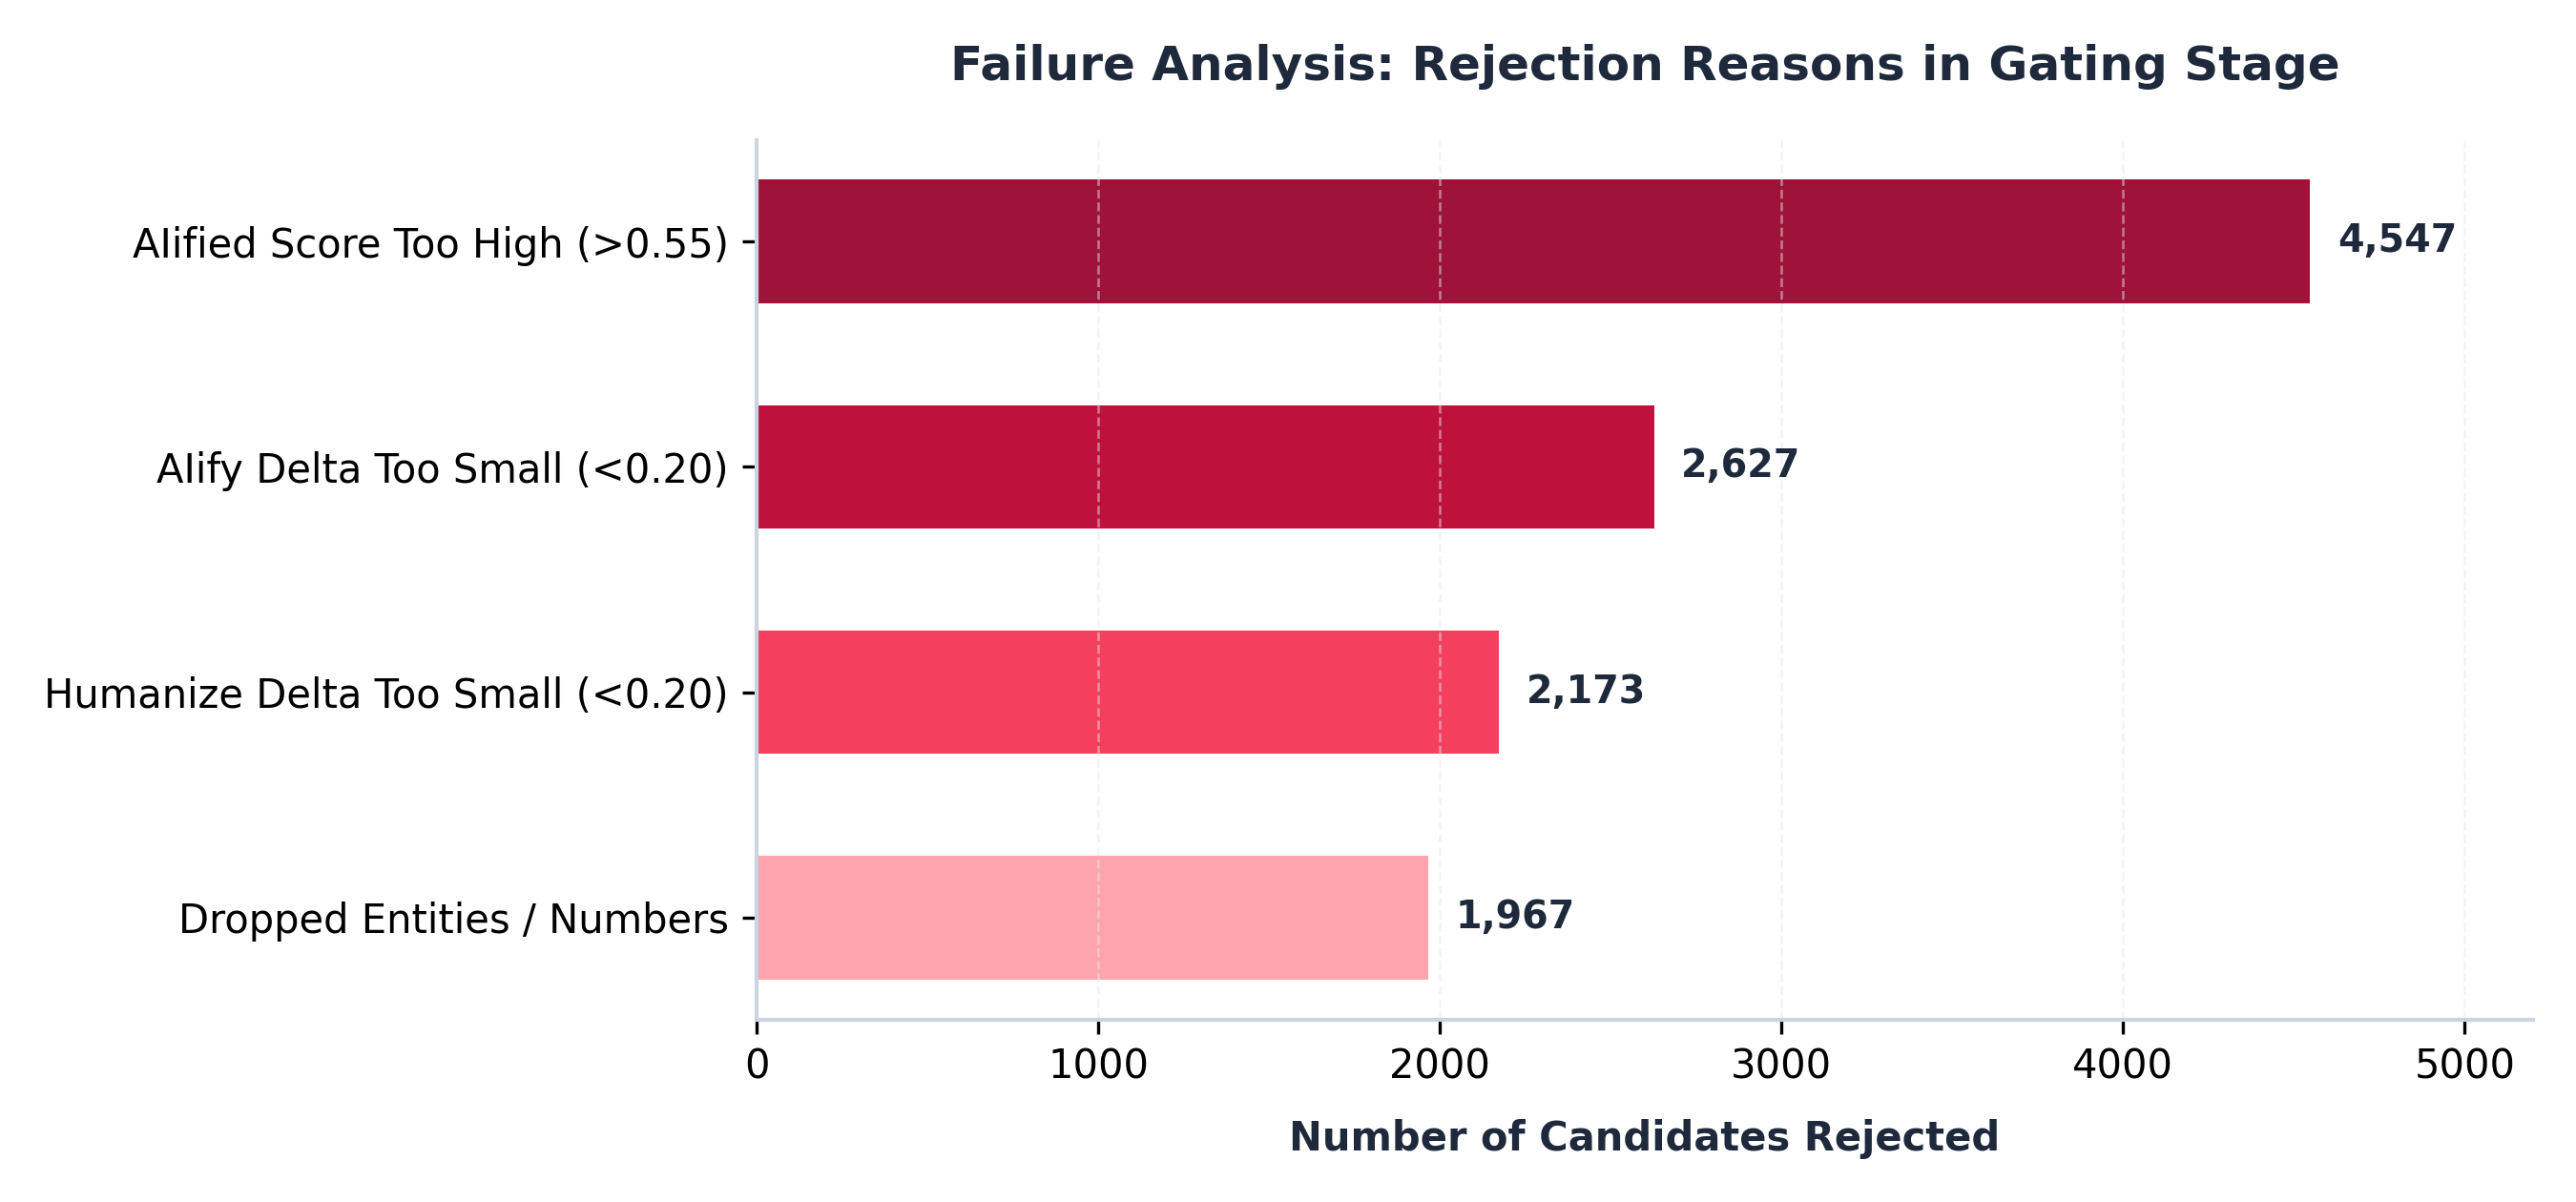
\includegraphics[width=0.75\textwidth]{figures/rejection_reasons.pdf}
\caption{Failure analysis breakdown of rejected candidate triples in the score-and-gate stage. Score thresholds (AIified score $> 0.55$ and small deltas) are the primary drivers of rejection, followed by entity preservation failures.}
\label{fig:rejection_reasons}
\end{figure}

\section{Discussion \& Limitations}
The empirical results demonstrate that two-layer stylometric gating is a viable pathway for scaling training data. However, several limitations and design trade-offs emerged during execution.

\subsection{Domain Imbalance}
The final accepted dataset is heavily skewed toward the \texttt{blog\_opinion} domain, which accounts for 50\% of the SFT pairs (523/1,045). In contrast, emails and creative writing represent less than 8\% combined. This imbalance is caused by the strictness of our preservation gates: creative writing and emails contain complex context formatting, highly specific names, and conversational structures that frequently trigger entity mismatches or length-ratio warnings. For downstream SFT training, practitioners should employ domain-balanced oversampling or adjust the gating thresholds dynamically per domain.

\subsection{Model Selection and Compute Trade-offs}
In initial pilots, we targeted the frontier model \texttt{google/gemini-3.1-pro-preview} for the humanization stage. However, at scale, the pro model suffered from high latency and frequent connection timeouts through OpenRouter, requiring over 5 hours for partial runs. By switching to \texttt{google/gemini-3-flash-preview} for humanization and \texttt{gemini-3.1-flash-lite-preview} for AIify, we completed the entire 8,000-sample pipeline in **35 minutes** with a 70\% reduction in token costs and only a single generation error, validating the use of fast, mid-tier models when coupled with strict offline filters.

\subsection{Reinforcement Learning Integration}
While this dataset serves as a high-quality SFT warm-up corpus, the ultimate objective of the Humanize-RL stack is reinforcement learning. By wrapping our Layer 1 deterministic scorer into a Gym-style environment using the PrimeIntellect \texttt{verifiers} package~\citep{verifiers}, we can compute token-level rewards dynamically during training. The reward function can be expressed as:
\begin{equation}
    Reward = Score_{L1} + \lambda \cdot Sim(x, x_{orig}) - \text{Penalty}_{drift}
\end{equation}
where $Sim$ is the semantic similarity (e.g., using sentence embeddings) and $\text{Penalty}_{drift}$ is a penalty triggered by number or entity drops. Because Layer 1 is deterministic and local, it can run directly in the RL training loop without slow API dependencies, enabling algorithms like GRPO or DAPO to run at scale.

\section{Conclusion \& Future Work}
We introduced Humanize-RL, a framework and pipeline that leverages a two-layer stylometric gating mechanism to build safe, high-quality, humanlike SFT instruction-tuning datasets. By isolating deterministic stylometric rules into a zero-cost local filter (Layer 1) and combining it with strict case-insensitive entity matching and proportional number tolerances, we scaled our corpus to 1,045 SFT pairs with high fidelity. Our evaluation demonstrates that our humanized rewrites achieve a human-vs-humanized AUROC of 0.398, matching human style distributions. Future work will explore training a Qwen3.5-9B model on the generated SFT dataset and executing GRPO training using our deterministic scorer as a reward verifier.

\bibliographystyle{abbrvnat}
\bibliography{references}

\end{document}
